\documentclass[prb,preprint]{revtex4-1} 
% The line above defines the type of LaTeX document.
% Note that AJP uses the same style as Phys. Rev. B (prb).

\usepackage{amsmath}  % needed for \tfrac, \bmatrix, etc.
\usepackage{amsfonts} % needed for bold Greek, Fraktur, and blackboard bold
\usepackage{graphicx} % needed for figures
\usepackage{color}
\usepackage{ulem}
\begin{document}

% Be sure to use the \title, \author, \affiliation, and \abstract macros
% to format your title page.  Don't use lower-level macros to  manually
% adjust the fonts and centering.

\title{Single-Photon Interference}


\author{Liza Mulder}
\email{emulder@smith.edu}
\affiliation{Department of Physics, Smith College, Northampton, MA 01063}


\author{Isabel Lipartio}
\email{iliparti@smith.edu}
\affiliation{Department of Physics, Smith College, Northampton, MA 01063}


\date{\today}



\begin{abstract}

It has been understood since the 19th century that light displays both wavelike and particle-like properties.  Light beams of differing phase interfere with each other and create observable light and dark fringes, as seen in Young's Double Slit experiment.  At the same time, light can be seen as a particle:  quanta of light, or photons, excite electrons to higher states of energy as seen in the photoelectric effect.  It is unlawful to attempt to classify light as a single entity.  We demonstrate the dual nature of light in the Single Photon Interference Experiment- a variation of Young's Double Slit Experiment.  We use a beam of light and a double slit apparatus, however, in this case, we have confirmation that, within a certain probability, there is only a single photon in flight through the double slit device at any time.  Considering light to be a particle, we would expect to see two single bright fringes projected onto a screen.  However, we do actually see an interference pattern as seen in the Double Slit experiment.  The photons 'interfered with themselves'- the light was both a wave and a particle at once!  In this paper, we discuss the revolutionary implications of this result as well as how we might model these interference patterns.  We fit the Fresnel and Fraunhofer models of interference to our data and discuss the advantages and disadvantages of each.

\end{abstract}

\maketitle % title page is now complete


\section{Introduction} % Section titles are automatically converted to all-caps.
% Section numbering is automatic.

The revolutionary discovery of the dual wave-particle nature of light has been of significance beginning in the 19th century and continuing to today.  Isaac Newton himself believed defining light as a particle-like quantity (calling them corpuscles) would explain light refraction and reflection \cite{newton}.  This idea was, however, superseded in the 19th century by the wave theory of light, due to the significant advances in electromagnetism.  The interference experiments by Young in the early 19th century opposed the ideas of Newton and demonstrated the wavelike nature of light.  Young sent light beams through a single slit and observed diffraction of light waves passing through the slit.  Young sent light beams through two slits and observed resultant interference patterns.  In the latter part of the 19th century, discoveries by Maxwell, Faraday, and Hertz lead to the unification of the theories of electricity and magnetism.  There is a single electromagnetic entity- an electromagnetic wave propagating through the electromagnetic field.  Light was realized to be an electromagnetic wave- a disturbance in an electromagnetic field.  The contemporary theories of light bore little resemblance to the corpuscular theory of Newton.  \cite{david}

However, support for the particle nature of light made a comeback in the early 20th century.  Perhaps the most famous example of this is Einstein's Nobel Prize winning explanation of the photoelectric effect, whose effects absolutely contradicted all predictions from the wave theory of light.  Einstein demonstrated that quanta of light, now called photons, strike the surface of a metal plate and excite electrons to freedom (Cite our modern physics book).  The advent of quantum mechanics- a field based largely off the quantized nature of electromagnetic energy, further explored the particle-like properties of light.  A further example of this is Compton Scattering- a effect where a photon elastically collides with an electron and experiences a shift in wavelength.  

We know now that we can treat light as a particle- photons scatter and collide with matter.  We can also treat it as a wave- light beams constructively and deconstructively interfere with each other.  But, particularly as relatively new physics students, can we call this an acceptable definition of light?  Can we say that we understand light?  The best way to test our understanding and perhaps obfuscate things a little bit is to undertake the Single Photon Interference Experiment.  We will take the same general set up as for the Young Double Slit Experiment:  beam of light, double slit, and means of viewing the output (see Methods section for a detailed description).  However, this time, we will reduce the intensity of light that we can be sure, to within a certain probability, that there is only a single photon in flight through the d


\section{Methods}

We used the Teach-Spin "2-Slit Interference One Photon at a Time" Apparatus for this experiment.  The apparatus comes with a long black box containing an adjustable light source (with green filter to restrict wavelength and intensity), a 670nm laser source for alignment, four magnetic slit-holders along the length of the box for adding slits in the path of the light, and two detector options at the end: a photodiode (for laser light) and a photomultiplier tube (for lightbulb illumination).  We placed a single columnating slit in the first holder to focus the light from the lightbulb. This created vertical a single-slit diffraction pattern, which we centered on the next set of slits.  In the second slit holder, in the middle of the box, we placed the double-slit, and immediately following that we placed the slit blocker (a wide single-slit) so we could choose to allow light through one slit, both slits, or neither.  At the far end of the box we placed a single slit for the detector slit - by moving this slit holder lengthwise across the channel we could "scan" the interference pattern and measure photon counts at regular intervals.  

Behind the detector slit was a photomultiplier tube (PMT).  A PMT generates an electrical current


\begin{figure}[h!]
\centering
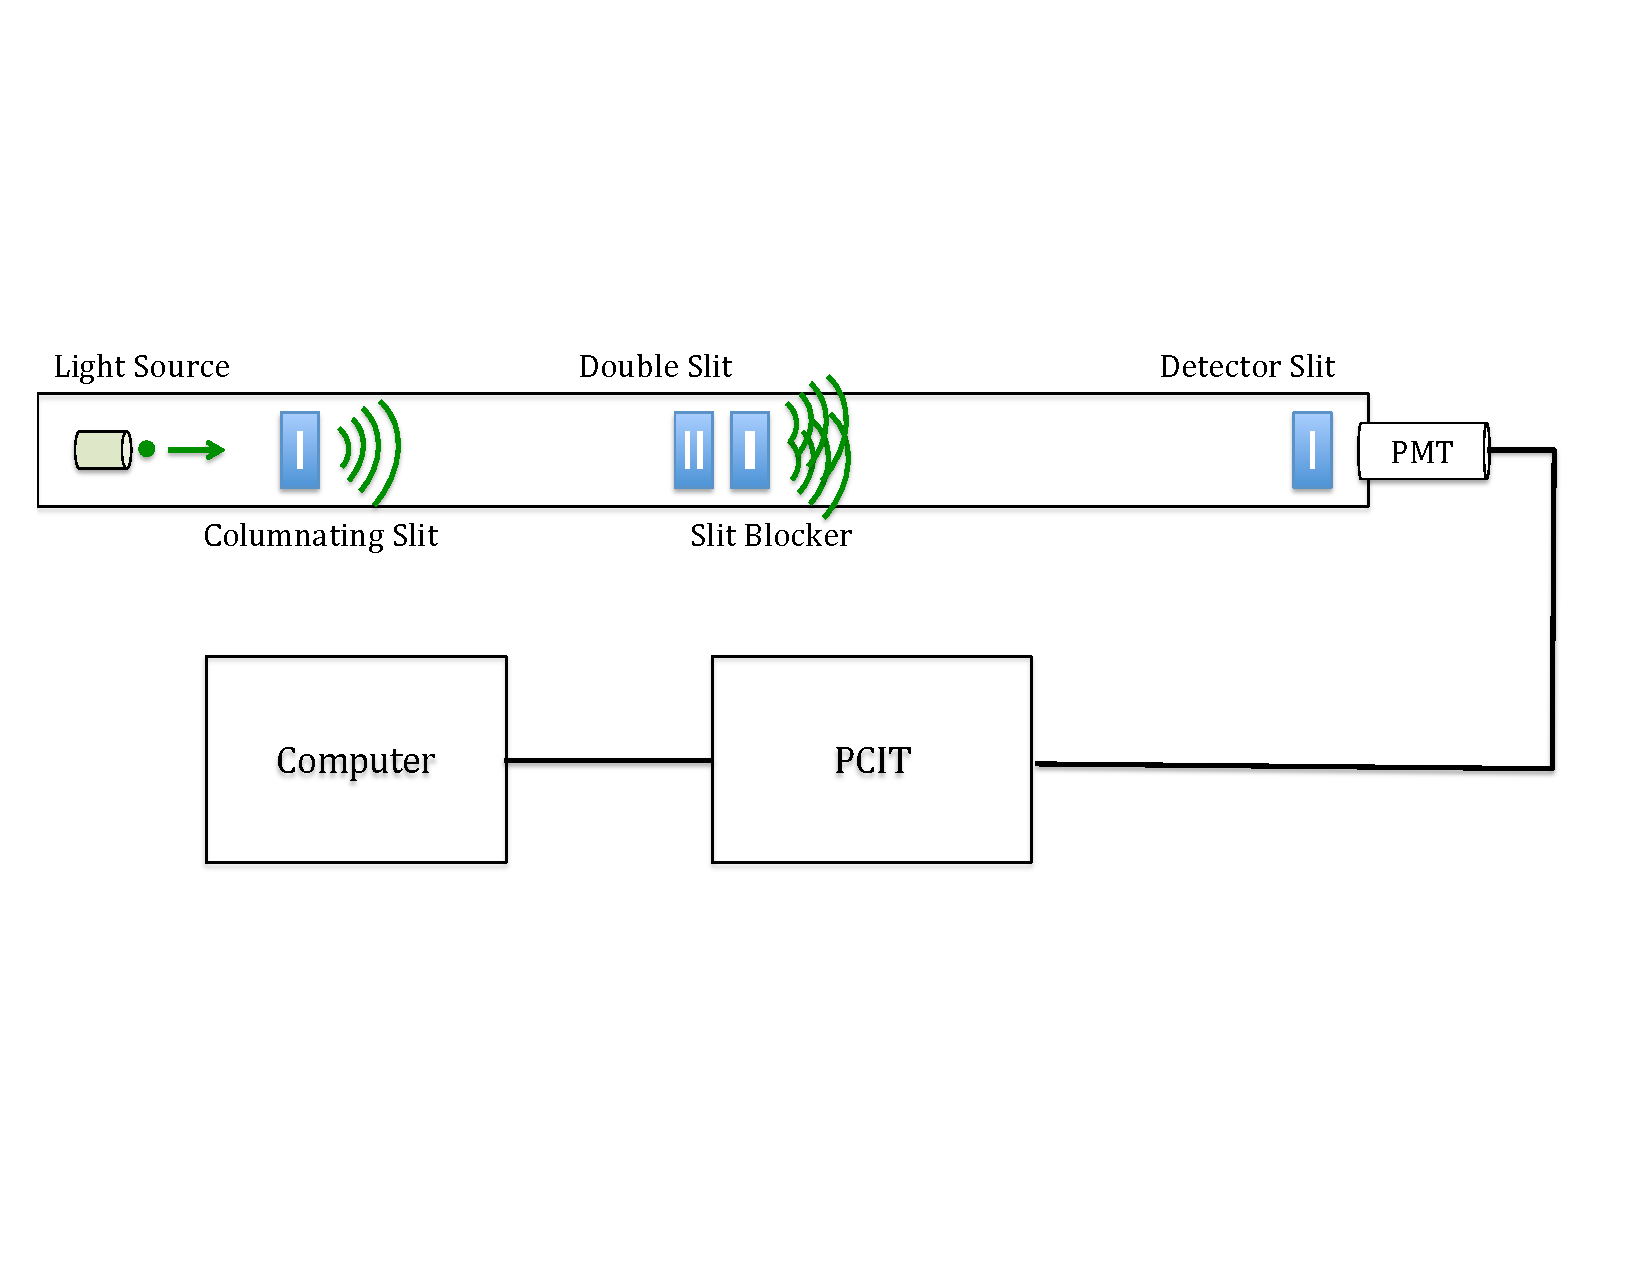
\includegraphics[width=6in]{set-up.pdf}
\caption{Teach-Spin apparatus to measure quantum interference: a 1m-long black box containing an adjustable light source (450nm), columnating single slit, double slit, slit blocker, detector slit, and photomultiplier tube (PMT) detector. We sent the PMT output to a pulse-counter interval timer (PCIT), and from there to the computer.}
\label{set-up}
\end{figure}





\section{Results}



\section{Analysis}

\begin{figure}[h!]
\centering
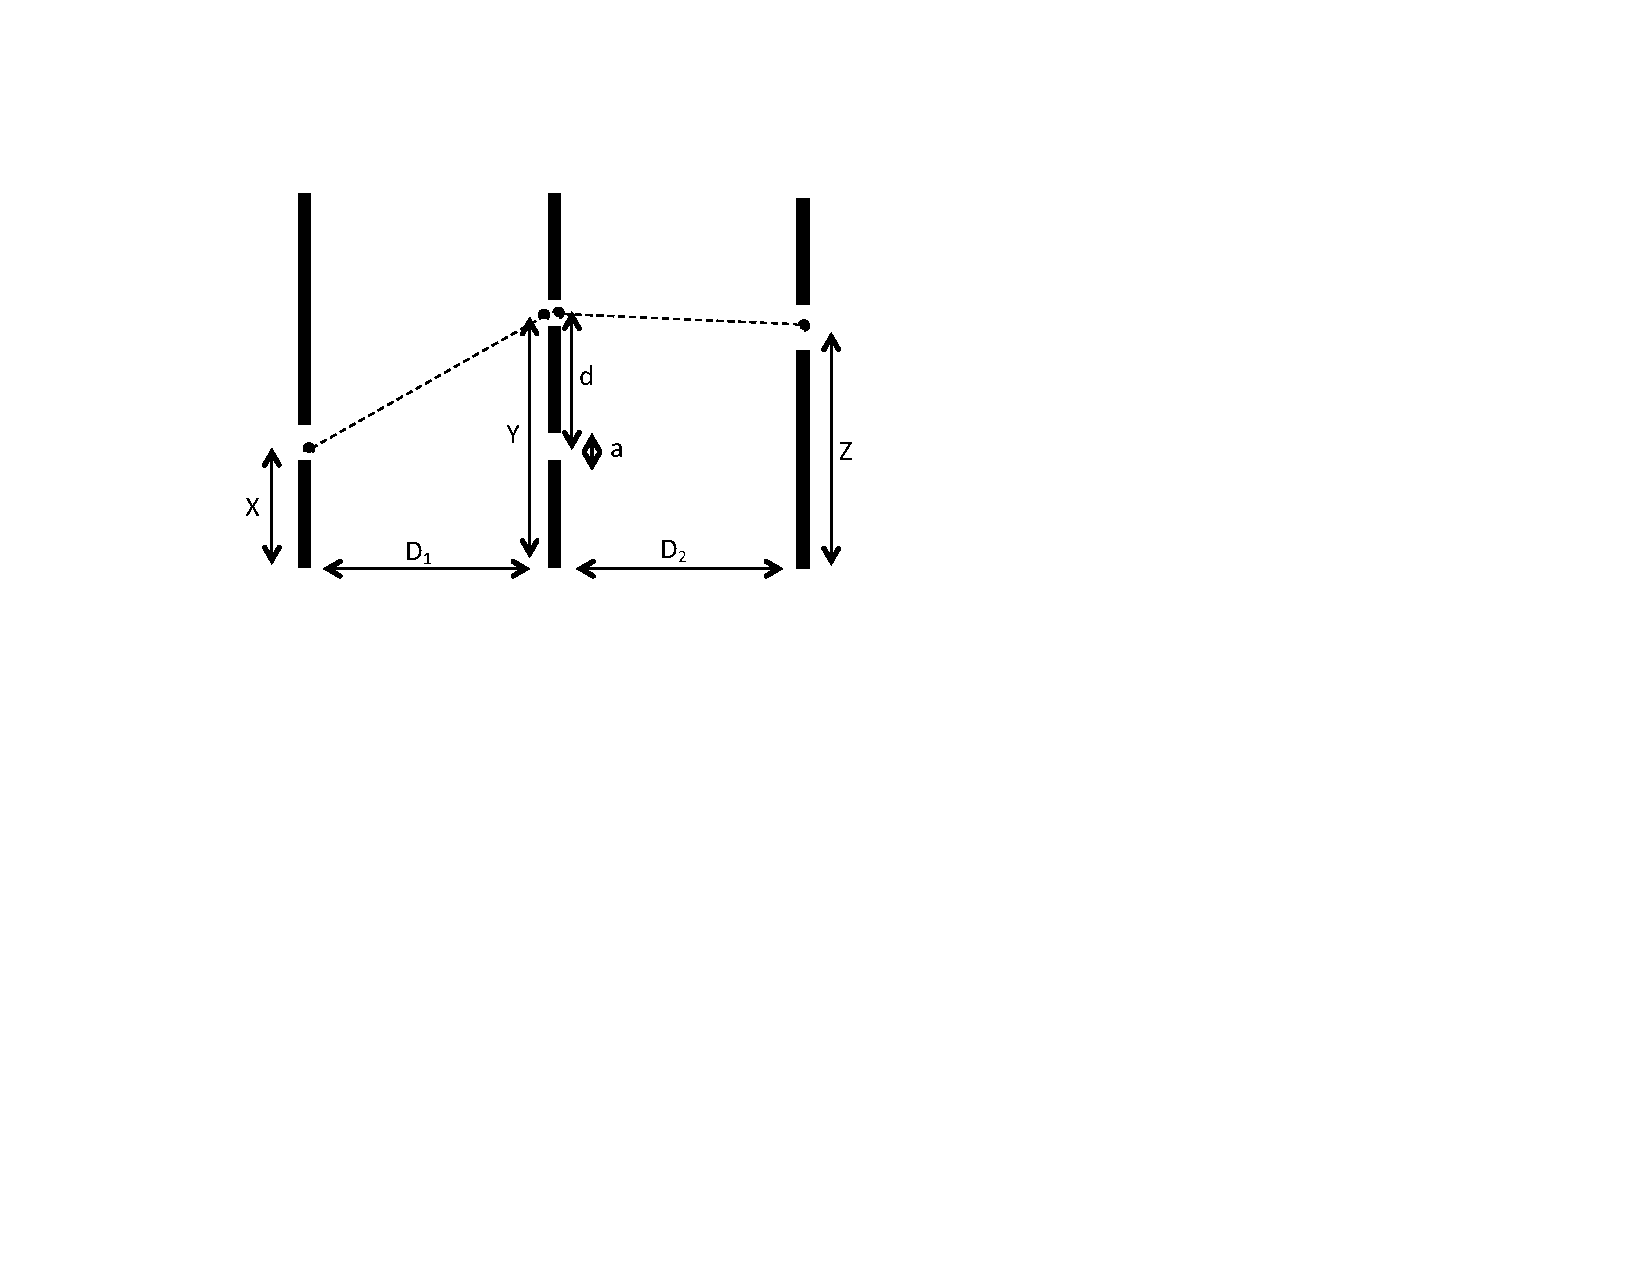
\includegraphics[width=6in]{fresnel_diagram.png}
\caption{The set-up and variables used in the Fresnel Approximation. Note that the variable "Z" in the fresnel formula is what we've been calling "X" in our other calculations - the position of the detector slit.}
\label{fresnel_diagram}
\end{figure}

\section{Discussion}

\section{Conclusion}

 
\begin{thebibliography}{3}
 \bibitem{newton}Use of Hamilton's Canonical Equations to Rectify Newton's Corpuscular Theory of Light:  A Missed Opportunity.  Buenker et al, 2004.  Sov. J. Chem. Phys. 22 (2003) 124
 \bibitem{david}Introduction to Electrodynamics, 4th Edition.  David J. Griffiths, 2012.  Addison Wesley.

\end{thebibliography}
\end{document}
